%%%%%%%%%%%%%%%%%%%%%%%%%%%%%%%%%%%%%%%%%%%%%%%%%%%%%%%%%%%%%%%%%%%%%%%%
%%%  THIS TEX FILE IS TO GENERATE PDF FILE FOR 
%%% 
%%%  COPYRIGHT (C) JIMMY LIN, 2013, UT AUSTIN
%%%%%%%%%%%%%%%%%%%%%%%%%%%%%%%%%%%%%%%%%%%%%%%%%%%%%%%%%%%%%%%%%%%%%%%%
\documentclass[11pt,a4paper]{article}
%%%%%%%%%%%%%%%%%%%%%%%%%%%%%%%%%%%%%%%%%%%%%%%%%%%%%%%%%%%%%%%%%%%%%%%%
%%%  PACKAGES USED IN THIS TEX SOURCE FILE
%%%%%%%%%%%%%%%%%%%%%%%%%%%%%%%%%%%%%%%%%%%%%%%%%%%%%%%%%%%%%%%%%%%%%%%%
\usepackage{geometry,amsthm,amsmath,graphicx,amssymb,fancyheadings}
\usepackage[]{mcode}
\usepackage[colorlinks,
            linkcolor=blue,
            anchorcolor=red,
            citecolor=green
            ]{hyperref}
% for my mac
\IfFileExists{/Users/JimmyLin/.latex/UTA_CS/JS.sty}{ 
    \usepackage{/Users/JimmyLin/.latex/UTA_CS/JS}
    \usepackage{/Users/JimmyLin/.latex/UTA_CS/JSASGN}
}{} 
% for UT's linux machine
\IfFileExists{/u/jimmylin/workspace/Configs/latex/UTA_CS/JS.sty}{
    \usepackage{/u/jimmylin/.latex/UTA_CS/JS} 
    \usepackage{/u/jimmylin/.latex/UTA_CS/JSASGN}
}{} 
%%%%%%%%%%%%%%%%%%%%%%%%%%%%%%%%%%%%%%%%%%%%%%%%%%%%%%%%%%%%%%%%%%%%%%%%
%%% MACROS CONTAINING THE FILE INFORMATION
%%%%%%%%%%%%%%%%%%%%%%%%%%%%%%%%%%%%%%%%%%%%%%%%%%%%%%%%%%%%%%%%%%%%%%%%
\renewcommand{\COURSE}{EE381V Large Scale Optimization}
\renewcommand{\LECTURER}{Sujay Sanghavi}
\renewcommand{\SECTION}{17350}
\renewcommand{\TASK}{Problem Set 2}
\renewcommand{\RELEASEDATE}{September 12, 2014}
\renewcommand{\DUEDATE}{September 18, 2014}
\renewcommand{\TIMECONSUME}{10 hours}
%%%%%%%%%%%%%%%%%%%%%%%%%%%%%%%%%%%%%%%%%%%%%%%%%%%%%%%%%%%%%%%%%%%%%%%%
%%% DOCUMENTATION STARTS FROM HERE 
%%%%%%%%%%%%%%%%%%%%%%%%%%%%%%%%%%%%%%%%%%%%%%%%%%%%%%%%%%%%%%%%%%%%%%%%
\begin{document}
%%%%%%%%%%%%%%%%%%%%%%%%%%%%%%%%%%%%%%%%%%%%%%%%%%%%%%%%%%%%%%%%%%%%%%%%
%% TITLE PAGE
%%%%%%%%%%%%%%%%%%%%%%%%%%%%%%%%%%%%%%%%%%%%%%%%%%%%%%%%%%%%%%%%%%%%%%%%
\begin{titlepage}
    \maketitle
\end{titlepage}
%%%%%%%%%%%%%%%%%%%%%%%%%%%%%%%%%%%%%%%%%%%%%%%%%%%%%%%%%%%%%%%%%%%%%%%%
%% CONTENT PAGE: TABLEOFCONTENTS, LISTOFTABLES, LIST OF FIGURES
%%%%%%%%%%%%%%%%%%%%%%%%%%%%%%%%%%%%%%%%%%%%%%%%%%%%%%%%%%%%%%%%%%%%%%%%
\renewcommand{\contentsname}{Table of Contents}
\begin{center} 
    \tableofcontents 
    %\listoftables 
    \listoffigures
\end{center}
\newpage
%%%%%%%%%%%%%%%%%%%%%%%%%%%%%%%%%%%%%%%%%%%%%%%%%%%%%%%%%%%%%%%%%%%%%%%%
%%% GENERAL DOCUMENTATION BEGINS 
%%%%%%%%%%%%%%%%%%%%%%%%%%%%%%%%%%%%%%%%%%%%%%%%%%%%%%%%%%%%%%%%%%%%%%%%

\section{Matlab and Computational Assignment}
\subsection{Five flavors for Eq. (9.20) in B \& V}
\subsubsection{Standard Gradient Descent with Backtracking}
{\bf Command} to be executed in matlab:
\begin{verbatim}
  >> x_init = [1 1]'; alpha = 0.3; bta = 0.8;
  >> [x, iter, all_costs] = gd_btls(x_init, @func, @func_grad, alpha, bta);
\end{verbatim}
{\bf Dump}
\begin{verbatim}
  Iter: 1, Cost: 5.292007e+00, Conv_Rate: 0.106142, gamma: 0.800000
  Iter: 2, Cost: 3.936296e+00, Conv_Rate: 0.743819, gamma: 0.409600
  Iter: 3, Cost: 3.440868e+00, Conv_Rate: 0.874138, gamma: 0.327680
  Iter: 4, Cost: 3.047567e+00, Conv_Rate: 0.885697, gamma: 0.262144
  Iter: 5, Cost: 2.851476e+00, Conv_Rate: 0.935657, gamma: 0.262144
  Iter: 6, Cost: 2.698084e+00, Conv_Rate: 0.946206, gamma: 0.209715
  Iter: 7, Cost: 2.621951e+00, Conv_Rate: 0.971783, gamma: 0.134218
  Iter: 8, Cost: 2.589490e+00, Conv_Rate: 0.987619, gamma: 0.107374
  Iter: 9, Cost: 2.571558e+00, Conv_Rate: 0.993075, gamma: 0.068719
                                ...
                                ...
  Iter: 40, Cost: 2.559267e+00, Conv_Rate: 1.000000, gamma: 0.000000
  Iter: 41, Cost: 2.559267e+00, Conv_Rate: 1.000000, gamma: 0.000000
  Iter: 42, Cost: 2.559267e+00, Conv_Rate: 1.000000, gamma: 0.000000
  Iter: 43, Cost: 2.559267e+00, Conv_Rate: 1.000000, gamma: 0.000000
  Iter: 44, Cost: 2.559267e+00, Conv_Rate: 1.000000, gamma: 0.000000
  Convergence reached!
\end{verbatim}
{\bf Minima}
\begin{verbatim}
    x = [-0.3379, -0.0031], obj = 2.559267 
   \end{verbatim}
{\bf Plot}
\begin{figure}[h]
    \centering
    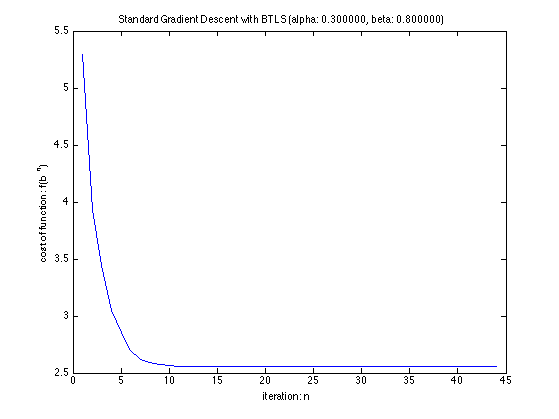
\includegraphics[width=5in,height=3in]{../ps2_matlab/1.png}
    \caption{Standard gradient descent with BTLS on
        Eq. 9.20 with $\alpha = 0.3$ and $\beta = 0.8$}
\end{figure}

\newpage
\subsubsection{Steepest Descent with $P_1$}
{\bf Command} to be executed in matlab:
\begin{verbatim}
  >> P1 = [8 0; 0 2];
  >> x_init = [1 1]'; alpha = 0.3; bta = 0.8;
  >> [x, iter, all_costs] = sd_btls(x_init, @func, @func_grad, P1, alpha, bta);
\end{verbatim}
{\bf Dump}
\begin{verbatim}
  Iter: 1, Cost: 4.109800e+00, Conv_Rate: 0.082430, gamma: 0.035184
  Iter: 2, Cost: 2.574134e+00, Conv_Rate: 0.626340, gamma: 0.409600
  Iter: 3, Cost: 2.561394e+00, Conv_Rate: 0.995051, gamma: 1.000000
  Iter: 4, Cost: 2.559319e+00, Conv_Rate: 0.999190, gamma: 0.800000
  Iter: 5, Cost: 2.559268e+00, Conv_Rate: 0.999980, gamma: 0.800000
  Iter: 6, Cost: 2.559267e+00, Conv_Rate: 1.000000, gamma: 0.800000
  Iter: 7, Cost: 2.559267e+00, Conv_Rate: 1.000000, gamma: 0.800000
  Iter: 8, Cost: 2.559267e+00, Conv_Rate: 1.000000, gamma: 0.800000
  Iter: 9, Cost: 2.559267e+00, Conv_Rate: 1.000000, gamma: 0.800000
  Iter: 10, Cost: 2.559267e+00, Conv_Rate: 1.000000, gamma: 0.800000
  Iter: 11, Cost: 2.559267e+00, Conv_Rate: 1.000000, gamma: 0.800000
  Iter: 12, Cost: 2.559267e+00, Conv_Rate: 1.000000, gamma: 1.000000
  Convergence reached!
\end{verbatim}
{\bf Minima}
\begin{verbatim}
    x = [-0.3466 -0.0000], obj = 2.559267 
   \end{verbatim}
{\bf Plot}
\begin{figure}[h]
    \centering
    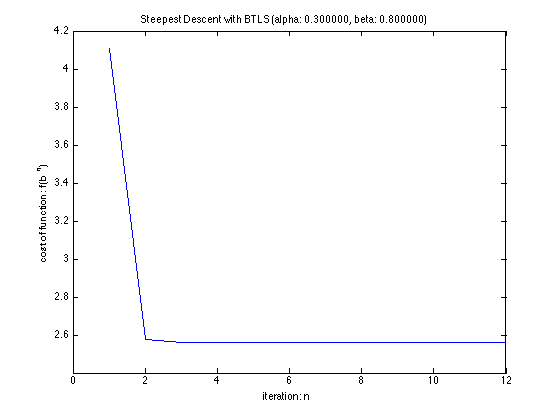
\includegraphics[width=5in,height=3in]{../ps2_matlab/2.png}
    \caption{Steepest Descent with BTLS on
        Eq. 9.20 with $P_1$, $\alpha = 0.3$ and $\beta = 0.8$}
\end{figure}

\newpage \subsubsection{Steepest Descent with $P_2$}
{\bf Command} to be executed in matlab:
\begin{verbatim}
  >> P2 = [2 0; 0 8];
  >> x_init = [1 1]'; alpha = 0.3; bta = 0.8;
  >> [x, iter, all_costs] = sd_btls(x_init, @func, @func_grad, P2, alpha, bta);
\end{verbatim}
{\bf Dump}
\begin{verbatim}
  Iter: 1, Cost: 5.397521e+00, Conv_Rate: 0.108258, gamma: 0.011529
  Iter: 2, Cost: 4.867283e+00, Conv_Rate: 0.901763, gamma: 0.068719
  Iter: 3, Cost: 4.673428e+00, Conv_Rate: 0.960172, gamma: 0.107374
  Iter: 4, Cost: 4.447617e+00, Conv_Rate: 0.951682, gamma: 0.085899
  Iter: 5, Cost: 4.276423e+00, Conv_Rate: 0.961509, gamma: 0.134218
  Iter: 6, Cost: 4.100684e+00, Conv_Rate: 0.958905, gamma: 0.107374
  Iter: 7, Cost: 3.955941e+00, Conv_Rate: 0.964703, gamma: 0.134218
  Iter: 8, Cost: 3.820349e+00, Conv_Rate: 0.965724, gamma: 0.134218
  Iter: 9, Cost: 3.687908e+00, Conv_Rate: 0.965333, gamma: 0.134218
  Iter: 10, Cost: 3.560463e+00, Conv_Rate: 0.965442, gamma: 0.134218
  Iter: 11, Cost: 3.444372e+00, Conv_Rate: 0.967394, gamma: 0.134218
  Iter: 12, Cost: 3.347890e+00, Conv_Rate: 0.971989, gamma: 0.167772
  Iter: 13, Cost: 3.259404e+00, Conv_Rate: 0.973570, gamma: 0.167772
                                ...
                                ...
  Iter: 164, Cost: 2.559267e+00, Conv_Rate: 1.000000, gamma: 0.262144
  Iter: 165, Cost: 2.559267e+00, Conv_Rate: 1.000000, gamma: 0.409600
  Iter: 166, Cost: 2.559267e+00, Conv_Rate: 1.000000, gamma: 0.327680
  Iter: 167, Cost: 2.559267e+00, Conv_Rate: 1.000000, gamma: 0.262144
  Iter: 168, Cost: 2.559267e+00, Conv_Rate: 1.000000, gamma: 0.167772
  Convergence reached!
\end{verbatim}
{\bf Minima}
\begin{verbatim}
    x = [-0.3466 -0.0000], obj = 2.559267
   \end{verbatim}
{\bf Plot}
\begin{figure}[h]
    \centering
    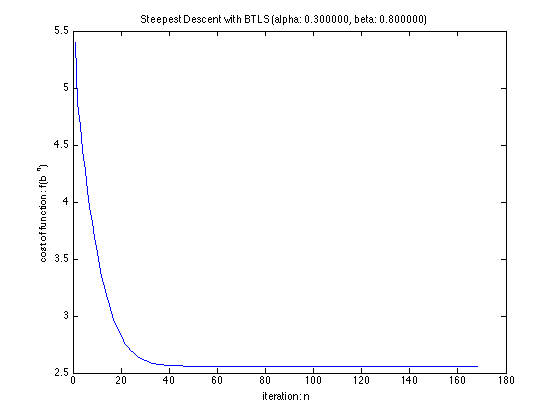
\includegraphics[width=5in,height=3in]{../ps2_matlab/3.png}
    \caption{Steepest Descent with BTLS on
        Eq. 9.20 with $P_2$, $\alpha = 0.3$ and $\beta = 0.8$}
\end{figure}

\newpage
\subsubsection{Cyclic Coordinate Descent}
{\bf Command} to be executed in matlab:
\begin{verbatim}
  >> x_init = [1 1]'; alpha = 0.3; bta = 0.8;
  >> [x, iter, all_costs] = ccd_btls(x_init, @func, @func_grad, alpha, bta);
\end{verbatim}
{\bf Dump}
\begin{verbatim}
  Iter: 1, Cost: 1.217687e+01, Conv_Rate: 0.244232, gamma: 0.043980
  Iter: 2, Cost: 3.551842e+00, Conv_Rate: 0.071239, gamma: 0.035184
  Iter: 3, Cost: 3.064142e+00, Conv_Rate: 0.862691, gamma: 0.209715
  Iter: 4, Cost: 2.732279e+00, Conv_Rate: 0.769257, gamma: 0.134218
  Iter: 5, Cost: 2.664867e+00, Conv_Rate: 0.975328, gamma: 0.209715
  Iter: 6, Cost: 2.600923e+00, Conv_Rate: 0.951925, gamma: 0.134218
  Iter: 7, Cost: 2.585633e+00, Conv_Rate: 0.994121, gamma: 0.262144
  Iter: 8, Cost: 2.563802e+00, Conv_Rate: 0.985727, gamma: 0.107374
  Iter: 9, Cost: 2.561867e+00, Conv_Rate: 0.999245, gamma: 0.209715
  Iter: 10, Cost: 2.560171e+00, Conv_Rate: 0.998584, gamma: 0.107374
  Iter: 11, Cost: 2.559836e+00, Conv_Rate: 0.999869, gamma: 0.167772
  Iter: 12, Cost: 2.559551e+00, Conv_Rate: 0.999758, gamma: 0.107374
  Iter: 13, Cost: 2.559478e+00, Conv_Rate: 0.999971, gamma: 0.167772
                                ...
                                ...
  Iter: 60, Cost: 2.559267e+00, Conv_Rate: 1.000000, gamma: 0.134218
  Iter: 61, Cost: 2.559267e+00, Conv_Rate: 1.000000, gamma: 0.262144
  Iter: 62, Cost: 2.559267e+00, Conv_Rate: 1.000000, gamma: 0.085899
  Iter: 63, Cost: 2.559267e+00, Conv_Rate: 1.000000, gamma: 0.327680
  Iter: 64, Cost: 2.559267e+00, Conv_Rate: 1.000000, gamma: 0.134218
  Convergence reached!
\end{verbatim}
{\bf Minima}
\begin{verbatim}
    x = [-0.3466 0.0000], obj = 2.559267 
   \end{verbatim}
{\bf Plot}
\begin{figure}[h]
    \centering
    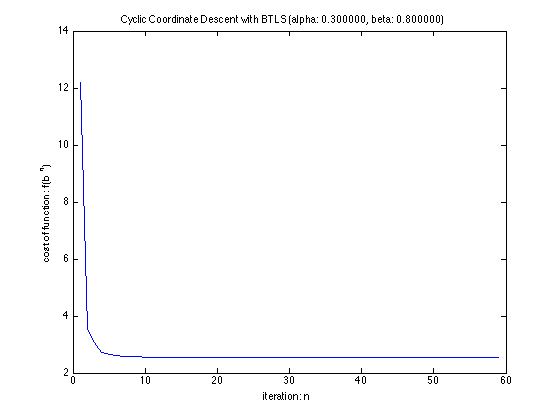
\includegraphics[width=5in,height=3in]{../ps2_matlab/4.png}
    \caption{Cyclical Coordinate Descent with BTLS on
        Eq. 9.20 with $\alpha = 0.3$ and $\beta = 0.8$}
\end{figure}
\newpage
\subsubsection{Greedy Coordinate Descent}
{\bf Command} to be executed in matlab:
\begin{verbatim}
  >> x_init = [1 1]'; alpha = 0.3; bta = 0.8;
  >> [x, iter, all_costs] = gcd_btls(x_init, @func, @func_grad, alpha, bta);
\end{verbatim}
{\bf Dump}
\begin{verbatim}
Iter: 1, Cost: 5.615225e+00, Conv_Rate: 0.112625, gamma: 0.005903
Iter: 2, Cost: 4.227075e+00, Conv_Rate: 0.752788, gamma: 0.028147
Iter: 3, Cost: 3.306101e+00, Conv_Rate: 0.782125, gamma: 0.035184
Iter: 4, Cost: 2.823271e+00, Conv_Rate: 0.853958, gamma: 0.054976
Iter: 5, Cost: 2.666299e+00, Conv_Rate: 0.944401, gamma: 0.068719
Iter: 6, Cost: 2.577867e+00, Conv_Rate: 0.966834, gamma: 0.107374
Iter: 7, Cost: 2.566546e+00, Conv_Rate: 0.995608, gamma: 0.107374
Iter: 8, Cost: 2.561822e+00, Conv_Rate: 0.998160, gamma: 0.107374
Iter: 9, Cost: 2.560570e+00, Conv_Rate: 0.999511, gamma: 0.107374
Iter: 10, Cost: 2.559369e+00, Conv_Rate: 0.999531, gamma: 0.107374
Iter: 11, Cost: 2.559298e+00, Conv_Rate: 0.999972, gamma: 0.107374
Iter: 12, Cost: 2.559277e+00, Conv_Rate: 0.999992, gamma: 0.107374
                                ...
                                ...
Iter: 32, Cost: 2.559267e+00, Conv_Rate: 1.000000, gamma: 0.107374
Iter: 33, Cost: 2.559267e+00, Conv_Rate: 1.000000, gamma: 0.107374
Iter: 34, Cost: 2.559267e+00, Conv_Rate: 1.000000, gamma: 0.107374
Iter: 35, Cost: 2.559267e+00, Conv_Rate: 1.000000, gamma: 0.107374
Convergence reached!
\end{verbatim}
{\bf Minima}
\begin{verbatim}
    x = [-0.3466 -0.0000], obj = 2.559267 
   \end{verbatim}
{\bf Plot}
\begin{figure}[h]
    \centering
    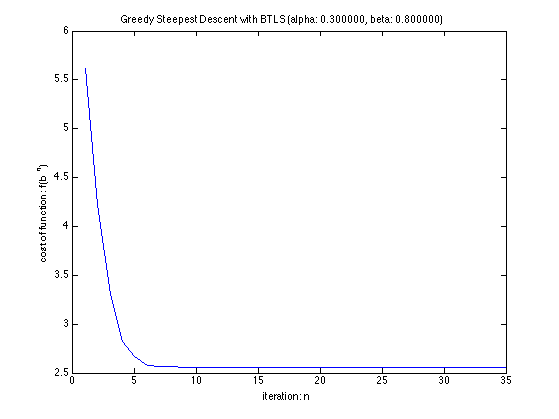
\includegraphics[width=5in,height=3in]{../ps2_matlab/5.png}
    \caption{Greedy Coordinate Descent with BTLS on
        Eq. 9.20 with $\alpha = 0.3$ and $\beta = 0.8$}
\end{figure}

\newpage
\subsubsection{Conclusions}
\begin{itemize}
    \item $(1, 1)$ is an decent initial point for all five
        flavors of optimization methods.
    \item Steepest descent method could both enhance and impair the convergence
        speed, comparing to standard gradient descent (uniform heuristic or
        unheuristic). The specific effect depends on what heuristic matrix is provided. 
    \item Greedy coordinate descent does converge to optima in less number of
        iterations than the cyclic cooridnate descent but in larger
        computational cost in each iteration.
\end{itemize}

\newpage
\section{Written Problems}
%\subsection{}


\newpage
\appendix
\section{Codes Printout}

\subsection{Eq. 20 and its gradient}
\lstinputlisting{../ps2_matlab/func.m}
\lstinputlisting{../ps2_matlab/func_grad.m}

\newpage
\subsection{Standard Gradient Descent with BackTracking Line Search}
\lstinputlisting{../ps2_matlab/gd_btls.m}
\newpage

\subsection{Steepest Descent with BackTracking Line Search}
\lstinputlisting{../ps2_matlab/sd_btls.m}
\newpage

\subsection{Cyclic Coordinate Descent}
\lstinputlisting{../ps2_matlab/ccd_btls.m}
\newpage

\subsection{Greedy Coordinate Descent}
\lstinputlisting{../ps2_matlab/gcd_btls.m}
\newpage
%%%%%%%%%%%%%%%%%%%%%%%%%%%%%%%%%%%%%%%%%%%%%%%%%%%%%%%%%%%%%%%%%%%%%%%%
%%% General Documentation ends
%%%%%%%%%%%%%%%%%%%%%%%%%%%%%%%%%%%%%%%%%%%%%%%%%%%%%%%%%%%%%%%%%%%%%%%%
\end{document}
\subsubsection{Steepest Descent with $P_2$}
